% Created by tikzDevice version 0.12.6 on 2026-08-01 05:44:22
% !TEX encoding = UTF-8 Unicode
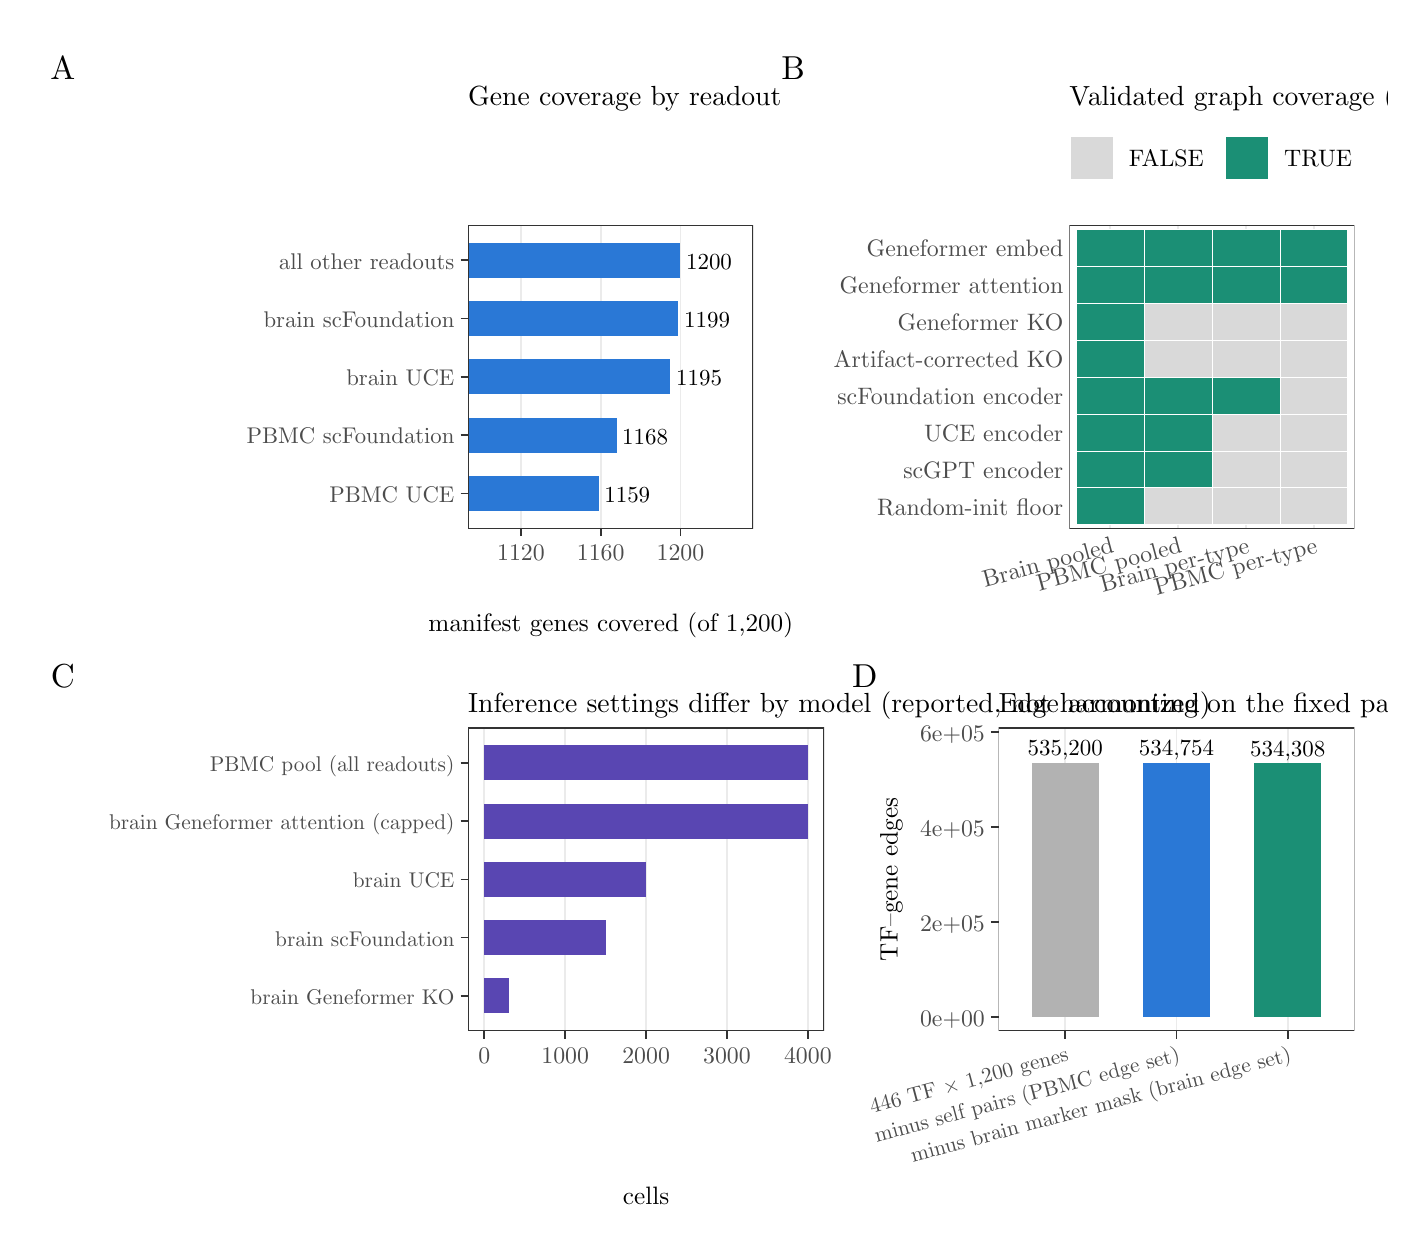
\begin{tikzpicture}[x=1pt,y=1pt]
\definecolor{fillColor}{RGB}{255,255,255}
\path[use as bounding box,fill=fillColor,fill opacity=0.00] (0,0) rectangle (491.44,433.62);
\begin{scope}
\path[clip] (  0.00,  0.00) rectangle (491.44,433.62);
\definecolor{drawColor}{RGB}{255,255,255}
\definecolor{fillColor}{RGB}{255,255,255}

\path[draw=drawColor,line width= 0.6pt,line join=round,line cap=round,fill=fillColor] ( -0.00,  0.00) rectangle (491.44,433.62);
\end{scope}
\begin{scope}
\path[clip] (  4.00,210.15) rectangle (268.18,429.62);
\definecolor{drawColor}{RGB}{255,255,255}
\definecolor{fillColor}{RGB}{255,255,255}

\path[draw=drawColor,line width= 0.6pt,line join=round,line cap=round,fill=fillColor] (  4.00,210.15) rectangle (268.18,429.62);
\end{scope}
\begin{scope}
\path[clip] (268.18,210.15) rectangle (485.44,429.62);
\definecolor{drawColor}{RGB}{255,255,255}
\definecolor{fillColor}{RGB}{255,255,255}

\path[draw=drawColor,line width= 0.6pt,line join=round,line cap=round,fill=fillColor] (268.18,210.15) rectangle (485.44,429.62);
\end{scope}
\begin{scope}
\path[clip] (159.16,252.67) rectangle (262.18,362.20);
\definecolor{fillColor}{RGB}{255,255,255}

\path[fill=fillColor] (159.16,252.67) rectangle (262.18,362.20);
\definecolor{drawColor}{gray}{0.92}

\path[draw=drawColor,line width= 0.6pt,line join=round] (178.25,252.67) --
	(178.25,362.20);

\path[draw=drawColor,line width= 0.6pt,line join=round] (207.07,252.67) --
	(207.07,362.20);

\path[draw=drawColor,line width= 0.6pt,line join=round] (235.88,252.67) --
	(235.88,362.20);
\definecolor{fillColor}{RGB}{42,120,214}

\path[fill=fillColor] (-628.61,301.12) rectangle (232.28,313.75);

\path[fill=fillColor] (-628.61,322.18) rectangle (235.16,334.82);

\path[fill=fillColor] (-628.61,280.05) rectangle (212.83,292.69);

\path[fill=fillColor] (-628.61,258.99) rectangle (206.34,271.63);

\path[fill=fillColor] (-628.61,343.24) rectangle (235.88,355.88);
\definecolor{drawColor}{RGB}{0,0,0}

\node[text=drawColor,anchor=base west,inner sep=0pt, outer sep=0pt, scale=  0.83] at (234.30,304.21) {1195};

\node[text=drawColor,anchor=base west,inner sep=0pt, outer sep=0pt, scale=  0.83] at (237.18,325.27) {1199};

\node[text=drawColor,anchor=base west,inner sep=0pt, outer sep=0pt, scale=  0.83] at (214.84,283.14) {1168};

\node[text=drawColor,anchor=base west,inner sep=0pt, outer sep=0pt, scale=  0.83] at (208.36,262.08) {1159};

\node[text=drawColor,anchor=base west,inner sep=0pt, outer sep=0pt, scale=  0.83] at (237.90,346.33) {1200};
\definecolor{drawColor}{gray}{0.20}

\path[draw=drawColor,line width= 0.6pt,line join=round,line cap=round] (159.16,252.67) rectangle (262.18,362.20);
\end{scope}
\begin{scope}
\path[clip] (  0.00,  0.00) rectangle (491.44,433.62);
\definecolor{drawColor}{gray}{0.30}

\node[text=drawColor,anchor=base east,inner sep=0pt, outer sep=0pt, scale=  0.82] at (154.21,262.12) {PBMC UCE};

\node[text=drawColor,anchor=base east,inner sep=0pt, outer sep=0pt, scale=  0.82] at (154.21,283.18) {PBMC scFoundation};

\node[text=drawColor,anchor=base east,inner sep=0pt, outer sep=0pt, scale=  0.82] at (154.21,304.24) {brain UCE};

\node[text=drawColor,anchor=base east,inner sep=0pt, outer sep=0pt, scale=  0.82] at (154.21,325.30) {brain scFoundation};

\node[text=drawColor,anchor=base east,inner sep=0pt, outer sep=0pt, scale=  0.82] at (154.21,346.37) {all other readouts};
\end{scope}
\begin{scope}
\path[clip] (  0.00,  0.00) rectangle (491.44,433.62);
\definecolor{drawColor}{gray}{0.20}

\path[draw=drawColor,line width= 0.6pt,line join=round] (156.41,265.31) --
	(159.16,265.31);

\path[draw=drawColor,line width= 0.6pt,line join=round] (156.41,286.37) --
	(159.16,286.37);

\path[draw=drawColor,line width= 0.6pt,line join=round] (156.41,307.43) --
	(159.16,307.43);

\path[draw=drawColor,line width= 0.6pt,line join=round] (156.41,328.50) --
	(159.16,328.50);

\path[draw=drawColor,line width= 0.6pt,line join=round] (156.41,349.56) --
	(159.16,349.56);
\end{scope}
\begin{scope}
\path[clip] (  0.00,  0.00) rectangle (491.44,433.62);
\definecolor{drawColor}{gray}{0.20}

\path[draw=drawColor,line width= 0.6pt,line join=round] (178.25,249.92) --
	(178.25,252.67);

\path[draw=drawColor,line width= 0.6pt,line join=round] (207.07,249.92) --
	(207.07,252.67);

\path[draw=drawColor,line width= 0.6pt,line join=round] (235.88,249.92) --
	(235.88,252.67);
\end{scope}
\begin{scope}
\path[clip] (  0.00,  0.00) rectangle (491.44,433.62);
\definecolor{drawColor}{gray}{0.30}

\node[text=drawColor,anchor=base,inner sep=0pt, outer sep=0pt, scale=  0.86] at (178.25,240.98) {1120};

\node[text=drawColor,anchor=base,inner sep=0pt, outer sep=0pt, scale=  0.86] at (207.07,240.98) {1160};

\node[text=drawColor,anchor=base,inner sep=0pt, outer sep=0pt, scale=  0.86] at (235.88,240.98) {1200};
\end{scope}
\begin{scope}
\path[clip] (  0.00,  0.00) rectangle (491.44,433.62);
\definecolor{drawColor}{RGB}{0,0,0}

\node[text=drawColor,anchor=base,inner sep=0pt, outer sep=0pt, scale=  0.91] at (210.67,215.36) {manifest genes covered (of 1,200)};
\end{scope}
\begin{scope}
\path[clip] (  0.00,  0.00) rectangle (491.44,433.62);
\definecolor{drawColor}{RGB}{0,0,0}

\node[text=drawColor,anchor=base west,inner sep=0pt, outer sep=0pt, scale=  1.00] at (159.16,405.53) {Gene coverage by readout};
\end{scope}
\begin{scope}
\path[clip] (  0.00,  0.00) rectangle (491.44,433.62);
\definecolor{drawColor}{RGB}{0,0,0}

\node[text=drawColor,anchor=base,inner sep=0pt, outer sep=0pt, scale=  1.20] at ( 12.74,414.80) {A};
\end{scope}
\begin{scope}
\path[clip] (376.42,252.67) rectangle (479.44,362.20);
\definecolor{fillColor}{RGB}{255,255,255}

\path[fill=fillColor] (376.42,252.67) rectangle (479.44,362.20);
\definecolor{drawColor}{gray}{0.92}

\path[draw=drawColor,line width= 0.6pt,line join=round] (391.13,252.67) --
	(391.13,362.20);

\path[draw=drawColor,line width= 0.6pt,line join=round] (415.66,252.67) --
	(415.66,362.20);

\path[draw=drawColor,line width= 0.6pt,line join=round] (440.19,252.67) --
	(440.19,362.20);

\path[draw=drawColor,line width= 0.6pt,line join=round] (464.72,252.67) --
	(464.72,362.20);
\definecolor{drawColor}{RGB}{255,255,255}
\definecolor{fillColor}{RGB}{27,143,117}

\path[draw=drawColor,line width= 0.2pt,fill=fillColor] (378.87,347.50) rectangle (403.40,360.86);

\path[draw=drawColor,line width= 0.2pt,fill=fillColor] (378.87,334.15) rectangle (403.40,347.50);

\path[draw=drawColor,line width= 0.2pt,fill=fillColor] (378.87,320.79) rectangle (403.40,334.15);

\path[draw=drawColor,line width= 0.2pt,fill=fillColor] (378.87,307.43) rectangle (403.40,320.79);

\path[draw=drawColor,line width= 0.2pt,fill=fillColor] (378.87,294.08) rectangle (403.40,307.43);

\path[draw=drawColor,line width= 0.2pt,fill=fillColor] (378.87,280.72) rectangle (403.40,294.08);

\path[draw=drawColor,line width= 0.2pt,fill=fillColor] (378.87,267.36) rectangle (403.40,280.72);

\path[draw=drawColor,line width= 0.2pt,fill=fillColor] (378.87,254.01) rectangle (403.40,267.36);

\path[draw=drawColor,line width= 0.2pt,fill=fillColor] (403.40,347.50) rectangle (427.93,360.86);

\path[draw=drawColor,line width= 0.2pt,fill=fillColor] (403.40,334.15) rectangle (427.93,347.50);
\definecolor{fillColor}{gray}{0.85}

\path[draw=drawColor,line width= 0.2pt,fill=fillColor] (403.40,320.79) rectangle (427.93,334.15);

\path[draw=drawColor,line width= 0.2pt,fill=fillColor] (403.40,307.43) rectangle (427.93,320.79);
\definecolor{fillColor}{RGB}{27,143,117}

\path[draw=drawColor,line width= 0.2pt,fill=fillColor] (403.40,294.08) rectangle (427.93,307.43);

\path[draw=drawColor,line width= 0.2pt,fill=fillColor] (403.40,280.72) rectangle (427.93,294.08);

\path[draw=drawColor,line width= 0.2pt,fill=fillColor] (403.40,267.36) rectangle (427.93,280.72);
\definecolor{fillColor}{gray}{0.85}

\path[draw=drawColor,line width= 0.2pt,fill=fillColor] (403.40,254.01) rectangle (427.93,267.36);
\definecolor{fillColor}{RGB}{27,143,117}

\path[draw=drawColor,line width= 0.2pt,fill=fillColor] (427.93,347.50) rectangle (452.46,360.86);

\path[draw=drawColor,line width= 0.2pt,fill=fillColor] (427.93,334.15) rectangle (452.46,347.50);
\definecolor{fillColor}{gray}{0.85}

\path[draw=drawColor,line width= 0.2pt,fill=fillColor] (427.93,320.79) rectangle (452.46,334.15);

\path[draw=drawColor,line width= 0.2pt,fill=fillColor] (427.93,307.43) rectangle (452.46,320.79);
\definecolor{fillColor}{RGB}{27,143,117}

\path[draw=drawColor,line width= 0.2pt,fill=fillColor] (427.93,294.08) rectangle (452.46,307.43);
\definecolor{fillColor}{gray}{0.85}

\path[draw=drawColor,line width= 0.2pt,fill=fillColor] (427.93,280.72) rectangle (452.46,294.08);

\path[draw=drawColor,line width= 0.2pt,fill=fillColor] (427.93,267.36) rectangle (452.46,280.72);

\path[draw=drawColor,line width= 0.2pt,fill=fillColor] (427.93,254.01) rectangle (452.46,267.36);
\definecolor{fillColor}{RGB}{27,143,117}

\path[draw=drawColor,line width= 0.2pt,fill=fillColor] (452.46,347.50) rectangle (476.98,360.86);

\path[draw=drawColor,line width= 0.2pt,fill=fillColor] (452.46,334.15) rectangle (476.98,347.50);
\definecolor{fillColor}{gray}{0.85}

\path[draw=drawColor,line width= 0.2pt,fill=fillColor] (452.46,320.79) rectangle (476.98,334.15);

\path[draw=drawColor,line width= 0.2pt,fill=fillColor] (452.46,307.43) rectangle (476.98,320.79);

\path[draw=drawColor,line width= 0.2pt,fill=fillColor] (452.46,294.08) rectangle (476.98,307.43);

\path[draw=drawColor,line width= 0.2pt,fill=fillColor] (452.46,280.72) rectangle (476.98,294.08);

\path[draw=drawColor,line width= 0.2pt,fill=fillColor] (452.46,267.36) rectangle (476.98,280.72);

\path[draw=drawColor,line width= 0.2pt,fill=fillColor] (452.46,254.01) rectangle (476.98,267.36);
\definecolor{drawColor}{gray}{0.20}

\path[draw=drawColor,line width= 0.6pt,line join=round,line cap=round] (376.42,252.67) rectangle (479.44,362.20);
\end{scope}
\begin{scope}
\path[clip] (  0.00,  0.00) rectangle (491.44,433.62);
\definecolor{drawColor}{gray}{0.30}

\node[text=drawColor,anchor=base east,inner sep=0pt, outer sep=0pt, scale=  0.86] at (374.22,257.32) {Random-init floor};

\node[text=drawColor,anchor=base east,inner sep=0pt, outer sep=0pt, scale=  0.86] at (374.22,270.67) {scGPT encoder};

\node[text=drawColor,anchor=base east,inner sep=0pt, outer sep=0pt, scale=  0.86] at (374.22,284.03) {UCE encoder};

\node[text=drawColor,anchor=base east,inner sep=0pt, outer sep=0pt, scale=  0.86] at (374.22,297.39) {scFoundation encoder};

\node[text=drawColor,anchor=base east,inner sep=0pt, outer sep=0pt, scale=  0.86] at (374.22,310.74) {Artifact-corrected KO};

\node[text=drawColor,anchor=base east,inner sep=0pt, outer sep=0pt, scale=  0.86] at (374.22,324.10) {Geneformer KO};

\node[text=drawColor,anchor=base east,inner sep=0pt, outer sep=0pt, scale=  0.86] at (374.22,337.46) {Geneformer attention};

\node[text=drawColor,anchor=base east,inner sep=0pt, outer sep=0pt, scale=  0.86] at (374.22,350.81) {Geneformer embed};
\end{scope}
\begin{scope}
\path[clip] (  0.00,  0.00) rectangle (491.44,433.62);
\definecolor{drawColor}{gray}{0.30}

\node[text=drawColor,rotate= 15.00,anchor=base east,inner sep=0pt, outer sep=0pt, scale=  0.86] at (392.88,243.96) {Brain pooled};

\node[text=drawColor,rotate= 15.00,anchor=base east,inner sep=0pt, outer sep=0pt, scale=  0.86] at (417.41,243.96) {PBMC pooled};

\node[text=drawColor,rotate= 15.00,anchor=base east,inner sep=0pt, outer sep=0pt, scale=  0.86] at (441.93,243.96) {Brain per-type};

\node[text=drawColor,rotate= 15.00,anchor=base east,inner sep=0pt, outer sep=0pt, scale=  0.86] at (466.46,243.96) {PBMC per-type};
\end{scope}
\begin{scope}
\path[clip] (  0.00,  0.00) rectangle (491.44,433.62);
\definecolor{fillColor}{RGB}{255,255,255}

\path[fill=fillColor] (371.00,373.20) rectangle (484.86,400.10);
\end{scope}
\begin{scope}
\path[clip] (  0.00,  0.00) rectangle (491.44,433.62);
\definecolor{fillColor}{RGB}{255,255,255}

\path[fill=fillColor] (376.50,378.70) rectangle (392.40,394.60);
\definecolor{drawColor}{RGB}{255,255,255}
\definecolor{fillColor}{gray}{0.85}

\path[draw=drawColor,line width= 0.2pt,fill=fillColor] (376.78,378.98) rectangle (392.11,394.31);
\end{scope}
\begin{scope}
\path[clip] (  0.00,  0.00) rectangle (491.44,433.62);
\definecolor{fillColor}{RGB}{255,255,255}

\path[fill=fillColor] (432.60,378.70) rectangle (448.50,394.60);
\definecolor{drawColor}{RGB}{255,255,255}
\definecolor{fillColor}{RGB}{27,143,117}

\path[draw=drawColor,line width= 0.2pt,fill=fillColor] (432.88,378.98) rectangle (448.21,394.31);
\end{scope}
\begin{scope}
\path[clip] (  0.00,  0.00) rectangle (491.44,433.62);
\definecolor{drawColor}{RGB}{0,0,0}

\node[text=drawColor,anchor=base west,inner sep=0pt, outer sep=0pt, scale=  0.86] at (397.90,383.28) {FALSE};
\end{scope}
\begin{scope}
\path[clip] (  0.00,  0.00) rectangle (491.44,433.62);
\definecolor{drawColor}{RGB}{0,0,0}

\node[text=drawColor,anchor=base west,inner sep=0pt, outer sep=0pt, scale=  0.86] at (454.00,383.28) {TRUE};
\end{scope}
\begin{scope}
\path[clip] (  0.00,  0.00) rectangle (491.44,433.62);
\definecolor{drawColor}{RGB}{0,0,0}

\node[text=drawColor,anchor=base west,inner sep=0pt, outer sep=0pt, scale=  1.00] at (376.42,405.53) {Validated graph coverage (coverage differs by tissue)};
\end{scope}
\begin{scope}
\path[clip] (  0.00,  0.00) rectangle (491.44,433.62);
\definecolor{drawColor}{RGB}{0,0,0}

\node[text=drawColor,anchor=base,inner sep=0pt, outer sep=0pt, scale=  1.20] at (276.56,414.80) {B};
\end{scope}
\begin{scope}
\path[clip] (  4.00,  3.00) rectangle (293.77,210.15);
\definecolor{drawColor}{RGB}{255,255,255}
\definecolor{fillColor}{RGB}{255,255,255}

\path[draw=drawColor,line width= 0.6pt,line join=round,line cap=round,fill=fillColor] (  4.00,  3.00) rectangle (293.77,210.15);
\end{scope}
\begin{scope}
\path[clip] (293.77,  3.00) rectangle (485.44,210.15);
\definecolor{drawColor}{RGB}{255,255,255}
\definecolor{fillColor}{RGB}{255,255,255}

\path[draw=drawColor,line width= 0.6pt,line join=round,line cap=round,fill=fillColor] (293.77,  3.00) rectangle (485.44,210.15);
\end{scope}
\begin{scope}
\path[clip] (159.16, 71.10) rectangle (287.77,180.62);
\definecolor{fillColor}{RGB}{255,255,255}

\path[fill=fillColor] (159.16, 71.10) rectangle (287.77,180.62);
\definecolor{drawColor}{gray}{0.92}

\path[draw=drawColor,line width= 0.6pt,line join=round] (165.00, 71.10) --
	(165.00,180.62);

\path[draw=drawColor,line width= 0.6pt,line join=round] (194.24, 71.10) --
	(194.24,180.62);

\path[draw=drawColor,line width= 0.6pt,line join=round] (223.47, 71.10) --
	(223.47,180.62);

\path[draw=drawColor,line width= 0.6pt,line join=round] (252.70, 71.10) --
	(252.70,180.62);

\path[draw=drawColor,line width= 0.6pt,line join=round] (281.93, 71.10) --
	(281.93,180.62);
\definecolor{fillColor}{RGB}{89,70,178}

\path[fill=fillColor] (165.00,140.60) rectangle (281.93,153.24);

\path[fill=fillColor] (165.00, 77.41) rectangle (173.77, 90.05);

\path[fill=fillColor] (165.00,119.54) rectangle (223.47,132.18);

\path[fill=fillColor] (165.00, 98.48) rectangle (208.85,111.11);

\path[fill=fillColor] (165.00,161.66) rectangle (281.93,174.30);
\definecolor{drawColor}{gray}{0.20}

\path[draw=drawColor,line width= 0.6pt,line join=round,line cap=round] (159.16, 71.10) rectangle (287.77,180.62);
\end{scope}
\begin{scope}
\path[clip] (  0.00,  0.00) rectangle (491.44,433.62);
\definecolor{drawColor}{gray}{0.30}

\node[text=drawColor,anchor=base east,inner sep=0pt, outer sep=0pt, scale=  0.77] at (154.21, 80.72) {brain Geneformer KO};

\node[text=drawColor,anchor=base east,inner sep=0pt, outer sep=0pt, scale=  0.77] at (154.21,101.78) {brain scFoundation};

\node[text=drawColor,anchor=base east,inner sep=0pt, outer sep=0pt, scale=  0.77] at (154.21,122.84) {brain UCE};

\node[text=drawColor,anchor=base east,inner sep=0pt, outer sep=0pt, scale=  0.77] at (154.21,143.91) {brain Geneformer attention (capped)};

\node[text=drawColor,anchor=base east,inner sep=0pt, outer sep=0pt, scale=  0.77] at (154.21,164.97) {PBMC pool (all readouts)};
\end{scope}
\begin{scope}
\path[clip] (  0.00,  0.00) rectangle (491.44,433.62);
\definecolor{drawColor}{gray}{0.20}

\path[draw=drawColor,line width= 0.6pt,line join=round] (156.41, 83.73) --
	(159.16, 83.73);

\path[draw=drawColor,line width= 0.6pt,line join=round] (156.41,104.80) --
	(159.16,104.80);

\path[draw=drawColor,line width= 0.6pt,line join=round] (156.41,125.86) --
	(159.16,125.86);

\path[draw=drawColor,line width= 0.6pt,line join=round] (156.41,146.92) --
	(159.16,146.92);

\path[draw=drawColor,line width= 0.6pt,line join=round] (156.41,167.98) --
	(159.16,167.98);
\end{scope}
\begin{scope}
\path[clip] (  0.00,  0.00) rectangle (491.44,433.62);
\definecolor{drawColor}{gray}{0.20}

\path[draw=drawColor,line width= 0.6pt,line join=round] (165.00, 68.35) --
	(165.00, 71.10);

\path[draw=drawColor,line width= 0.6pt,line join=round] (194.24, 68.35) --
	(194.24, 71.10);

\path[draw=drawColor,line width= 0.6pt,line join=round] (223.47, 68.35) --
	(223.47, 71.10);

\path[draw=drawColor,line width= 0.6pt,line join=round] (252.70, 68.35) --
	(252.70, 71.10);

\path[draw=drawColor,line width= 0.6pt,line join=round] (281.93, 68.35) --
	(281.93, 71.10);
\end{scope}
\begin{scope}
\path[clip] (  0.00,  0.00) rectangle (491.44,433.62);
\definecolor{drawColor}{gray}{0.30}

\node[text=drawColor,anchor=base,inner sep=0pt, outer sep=0pt, scale=  0.86] at (165.00, 59.41) {0};

\node[text=drawColor,anchor=base,inner sep=0pt, outer sep=0pt, scale=  0.86] at (194.24, 59.41) {1000};

\node[text=drawColor,anchor=base,inner sep=0pt, outer sep=0pt, scale=  0.86] at (223.47, 59.41) {2000};

\node[text=drawColor,anchor=base,inner sep=0pt, outer sep=0pt, scale=  0.86] at (252.70, 59.41) {3000};

\node[text=drawColor,anchor=base,inner sep=0pt, outer sep=0pt, scale=  0.86] at (281.93, 59.41) {4000};
\end{scope}
\begin{scope}
\path[clip] (  0.00,  0.00) rectangle (491.44,433.62);
\definecolor{drawColor}{RGB}{0,0,0}

\node[text=drawColor,anchor=base,inner sep=0pt, outer sep=0pt, scale=  0.91] at (223.47,  8.21) {cells};
\end{scope}
\begin{scope}
\path[clip] (  0.00,  0.00) rectangle (491.44,433.62);
\definecolor{drawColor}{RGB}{0,0,0}

\node[text=drawColor,anchor=base west,inner sep=0pt, outer sep=0pt, scale=  1.00] at (159.16,186.06) {Inference settings differ by model (reported, not harmonized)};
\end{scope}
\begin{scope}
\path[clip] (  0.00,  0.00) rectangle (491.44,433.62);
\definecolor{drawColor}{RGB}{0,0,0}

\node[text=drawColor,anchor=base,inner sep=0pt, outer sep=0pt, scale=  1.20] at ( 12.74,195.32) {C};
\end{scope}
\begin{scope}
\path[clip] (350.82, 71.10) rectangle (479.44,180.62);
\definecolor{fillColor}{RGB}{255,255,255}

\path[fill=fillColor] (350.82, 71.10) rectangle (479.44,180.62);
\definecolor{drawColor}{gray}{0.92}

\path[draw=drawColor,line width= 0.6pt,line join=round] (374.94, 71.10) --
	(374.94,180.62);

\path[draw=drawColor,line width= 0.6pt,line join=round] (415.13, 71.10) --
	(415.13,180.62);

\path[draw=drawColor,line width= 0.6pt,line join=round] (455.32, 71.10) --
	(455.32,180.62);
\definecolor{fillColor}{gray}{0.70}

\path[fill=fillColor] (362.88, 76.07) rectangle (386.99,167.95);
\definecolor{fillColor}{RGB}{42,120,214}

\path[fill=fillColor] (403.07, 76.07) rectangle (427.19,167.88);
\definecolor{fillColor}{RGB}{27,143,117}

\path[fill=fillColor] (443.26, 76.07) rectangle (467.38,167.80);
\definecolor{drawColor}{RGB}{0,0,0}

\node[text=drawColor,anchor=base,inner sep=0pt, outer sep=0pt, scale=  0.83] at (374.94,170.53) {535,200};

\node[text=drawColor,anchor=base,inner sep=0pt, outer sep=0pt, scale=  0.83] at (415.13,170.46) {534,754};

\node[text=drawColor,anchor=base,inner sep=0pt, outer sep=0pt, scale=  0.83] at (455.32,170.38) {534,308};
\definecolor{drawColor}{gray}{0.20}

\path[draw=drawColor,line width= 0.6pt,line join=round,line cap=round] (350.82, 71.10) rectangle (479.44,180.62);
\end{scope}
\begin{scope}
\path[clip] (  0.00,  0.00) rectangle (491.44,433.62);
\definecolor{drawColor}{gray}{0.30}

\node[text=drawColor,anchor=base east,inner sep=0pt, outer sep=0pt, scale=  0.86] at (345.87, 72.71) {0e+00};

\node[text=drawColor,anchor=base east,inner sep=0pt, outer sep=0pt, scale=  0.86] at (345.87,107.04) {2e+05};

\node[text=drawColor,anchor=base east,inner sep=0pt, outer sep=0pt, scale=  0.86] at (345.87,141.37) {4e+05};

\node[text=drawColor,anchor=base east,inner sep=0pt, outer sep=0pt, scale=  0.86] at (345.87,175.71) {6e+05};
\end{scope}
\begin{scope}
\path[clip] (  0.00,  0.00) rectangle (491.44,433.62);
\definecolor{drawColor}{gray}{0.20}

\path[draw=drawColor,line width= 0.6pt,line join=round] (348.07, 76.07) --
	(350.82, 76.07);

\path[draw=drawColor,line width= 0.6pt,line join=round] (348.07,110.41) --
	(350.82,110.41);

\path[draw=drawColor,line width= 0.6pt,line join=round] (348.07,144.74) --
	(350.82,144.74);

\path[draw=drawColor,line width= 0.6pt,line join=round] (348.07,179.08) --
	(350.82,179.08);
\end{scope}
\begin{scope}
\path[clip] (  0.00,  0.00) rectangle (491.44,433.62);
\definecolor{drawColor}{gray}{0.20}

\path[draw=drawColor,line width= 0.6pt,line join=round] (374.94, 68.35) --
	(374.94, 71.10);

\path[draw=drawColor,line width= 0.6pt,line join=round] (415.13, 68.35) --
	(415.13, 71.10);

\path[draw=drawColor,line width= 0.6pt,line join=round] (455.32, 68.35) --
	(455.32, 71.10);
\end{scope}
\begin{scope}
\path[clip] (  0.00,  0.00) rectangle (491.44,433.62);
\definecolor{drawColor}{gray}{0.30}

\node[text=drawColor,rotate= 15.00,anchor=base east,inner sep=0pt, outer sep=0pt, scale=  0.77] at (376.50, 60.32) {446 TF $\times$ 1,200 genes};

\node[text=drawColor,rotate= 15.00,anchor=base east,inner sep=0pt, outer sep=0pt, scale=  0.77] at (416.69, 60.32) {minus self pairs (PBMC edge set)};

\node[text=drawColor,rotate= 15.00,anchor=base east,inner sep=0pt, outer sep=0pt, scale=  0.77] at (456.88, 60.32) {minus brain marker mask (brain edge set)};
\end{scope}
\begin{scope}
\path[clip] (  0.00,  0.00) rectangle (491.44,433.62);
\definecolor{drawColor}{RGB}{0,0,0}

\node[text=drawColor,rotate= 90.00,anchor=base,inner sep=0pt, outer sep=0pt, scale=  0.91] at (314.35,125.86) {TF--gene edges};
\end{scope}
\begin{scope}
\path[clip] (  0.00,  0.00) rectangle (491.44,433.62);
\definecolor{drawColor}{RGB}{0,0,0}

\node[text=drawColor,anchor=base west,inner sep=0pt, outer sep=0pt, scale=  1.00] at (350.82,186.06) {Edge accounting on the fixed panel};
\end{scope}
\begin{scope}
\path[clip] (  0.00,  0.00) rectangle (491.44,433.62);
\definecolor{drawColor}{RGB}{0,0,0}

\node[text=drawColor,anchor=base,inner sep=0pt, outer sep=0pt, scale=  1.20] at (302.52,195.32) {D};
\end{scope}
\end{tikzpicture}
